% Contenidos del capítulo.
% Las secciones presentadas son orientativas y no representan
% necesariamente la organización que debe tener este capítulo.


% \subsubsection{2. Desarrollo de la Interfaz de Usuario}

% La interfaz de usuario desempeña un papel crucial en la usabilidad de la herramienta. Los objetivos relacionados con la interfaz de usuario incluyen:

% \begin{itemize}
%     \item Diseñar una interfaz de usuario intuitiva y fácil de usar para permitir a los usuarios configurar los parámetros de generación.
%     \item Implementar una interfaz de usuario que refleje de manera efectiva las opciones disponibles para la generación de terrenos.
% \end{itemize}

\section{Análisis}

\subsection{Objetivos de Implementación}

Los objetivos de implementación se centran en las metas técnicas y funcionales que se buscan alcanzar en el desarrollo de la herramienta de generación de terreno procedimental en Unity. Estos objetivos se dividen en los siguientes aspectos clave:

\subsubsection{1. Diseño de Algoritmos de Generación}

El objetivo principal en esta fase de implementación es diseñar algoritmos de generación de terreno eficientes que sean capaces de producir resultados convincentes. Esto incluye:

\begin{itemize}
    \item Investigar y seleccionar algoritmos de generación de terrenos adecuados para el proyecto.
    \item Diseñar algoritmos que permitan la creación de terrenos realistas y variados.
\end{itemize}

\subsubsection{2. Optimización del Rendimiento}

Para asegurar que la herramienta funcione eficientemente en diversas plataformas y escenarios de desarrollo, se establecen los siguientes objetivos: 

\begin{itemize}
    \item Optimizar el rendimiento de los algoritmos de generación para maximizar los fotogramas por segundo
    \item Implementar estrategias de cálculo paralelo utilizando el Job System de Unity para acelerar la generación de terreno.
\end{itemize}

\subsubsection{3. Pruebas y Validación}

La validación de la herramienta es fundamental para garantizar su correcto funcionamiento. Los objetivos relacionados con las pruebas son:

\begin{itemize}
    \item Detectar posibles errores y problemas de rendimiento. Mantener la coherencia entre fragmentos vecinos para crear terrenos continuos.
    \item Validar que la herramienta genera terrenos controlados de manera realista
    \item Comprobar que los resultados se integran visualmente en los juegos o proyectos de Unity y permiten la explorabilidad. 
\end{itemize}

\subsubsection{4. Mejoras en Realismo y Diferenciación de Alturas}

Además de los objetivos mencionados, se pretende mejorar el realismo de los terrenos generados mediante la implementación de algoritmos de erosión. Los objetivos adicionales incluyen:

\begin{itemize}
    \item Investigar y aplicar algoritmos de erosión para simular procesos geológicos en los terrenos generados.
    \item Evaluar cómo los algoritmos de erosión mejoran la apariencia y autenticidad de los terrenos.
    \item Implementar diferenciación de altura en los terrenos asignando colores basados en la elevación para una visualización más rica y comprensible.
\end{itemize}

\subsection{Requisitos del Sistema}

\subsubsection{Requisitos Funcionales}

\begin{enumerate}
    \item \textbf{Generación de Terrenos:} El sistema debe ser capaz de generar terrenos de forma procesal en tiempo real sin caídas o discontinuidades significativas en la velocidad de fotogramas.
    
    \item \textbf{Continuidad del terreno:} El terreno no debe tener discontinuidades y debe generar extensiones continuas sin transiciones perceptibles.
    
    \item \textbf{Configuración de propiedades:} Los usuarios deberían poder modificar el resultado final del terreno generado en función de los parámetros de entrada.
    
    \item \textbf{Optimización del Rendimiento:}El sistema debe tener un buen rendimiento en términos de fps y memoria caché, optimizando tanto espacial como temporalmente.
    
    \item \textbf{Erosión:} Se deben implementar algoritmos de erosión para mejorar la apariencia de los terrenos generados y proporcionar una apariencia más realista.
    
    \item \textbf{Diferenciación de Alturas:} El sistema debería asignar colores a los vértices en función de las distintas elevaciones del terreno para crear una apariencia más realista.
\end{enumerate}

\subsubsection{Requisitos No Funcionales}

\begin{enumerate}
    \item \textbf{Rendimiento:} El sistema debe tener la capacidad de generar terrenos en tiempo real sin experimentar retrasos notables en la ejecución.
    
    \item \textbf{Compatibilidad con Unity:} La herramienta debe integrarse perfectamente con el motor de Unity, aprovechando sus capacidades y recursos.
    
    \item \textbf{Portabilidad:} el sistema debe ser compatible con múltiples plataformas y versiones de Unity, permitiendo a los desarrolladores usarlo en varios proyectos.
    
    \item \textbf{Usabilidad:} El sistema debe ser intuitivo, con parámetros claramente nombrados que no confundan al usuario y expresen claramente su función.
    
    \item \textbf{Realismo Visual:} El sistema debe ser capaz de generar terrenos con realismo visual, incluyendo detalles naturales como montañas, valles.
    
    \item \textbf{Diferenciación de Alturas:} La herramienta debe permitir la diferenciación de alturas en el terreno mediante la asignación de colores o texturas específicas para representar diferentes elevaciones, facilitando la visualización y comprensión del terreno generado.

\end{enumerate}

\subsection{Arquitectura del Sistema}

\subsubsection{Visión General}
La arquitectura del sistema tiene un enfoque modular y consta de varios componentes interconectados. El sistema ha sido diseñado para ser realmente flexible y escalable, de manera que permita la generación procedural de terrenos de manera eficiente. La arquitectura se centra en la generación de terrenos y su visualización en tiempo real.

\subsubsection{Componentes del Sistema}
Los componentes clave del sistema incluyen:

\begin{itemize}
    \item \textbf{Generadores del terreno:} El terreno se generará mediante esta componente del sistema. Además, se encargará de crear la malla y de la gestión de la generación de mallas teniendo en cuento el movimiento del usuario por el espacio. Más tarde, en el diseño, veremos que esta componente se dividirá en varias partes.

    \item \textbf{Generadores de altura:} Tratarán las posiciones de la malla del terreno que se quiere generar, asignando alturas basándose en la generación de mapas de ruido en las coordeandas que corresponden al vértice.
    
    \item \textbf{Generador de erosión:} Esta componente se encarga de modoifcar el mapa de alturas produciendo así el efecto de erosión.
    
    \item \textbf{Jobs:} Serán parte de la implementación de los generadores de terreno y altura que permitirán paralelizar sus procesos.

    \item \textbf{Generador de texturas:} Esta componente se encargará de atribuir colores a los vértices para que se pueda percibir la diferencia de alturas de manera visual.    
        
    \item \textbf{Gestión de propiedades del terreno:} Se encargará de almacenar las configuraciones del sistema, incluyendo parámetros de generación de terrenos, configuraciones de malla y opciones de visualización.
\end{itemize}

Con esta arquitectura modular y bien definida conseguirmos una generación procedural de terrenos que sea flexible y eficaz en Unity.

\subsubsection{Diagramas de Arquitectura}
A continuación, se presentan unos diagramas de arquitectura en los que se muestra la estructura y las relaciones que existen entre los componentes del sistema:

\subsubsection{Diagrama de Casos de Uso}

Para ser capaces decomprender mejor las interacciones entre el sistema y los usuarios, se han creado diagramas de casos de uso. Estos diagramas describen la forma en la que los usuarios interactúan con el sistema y las funcionalidades que están disponibles para ellos.

\begin{figure}[H]
    \centering
    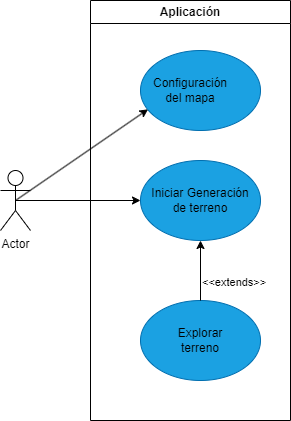
\includegraphics[width=0.5\textwidth]{img/UseCases.png}
    \caption{Diagrama de Casos de Uso del Proyecto.}
\end{figure}

\newpage
\subsubsection{Diagrama de Flujo}

En el diagrama de flujo se detalla, de manera general y apropiada la fase de análisis, los pasos y el flujo de las instrucciones que tendrán que llevarse a cabo para la generación infinita de terreno.

\begin{figure}[H]
    \centering
    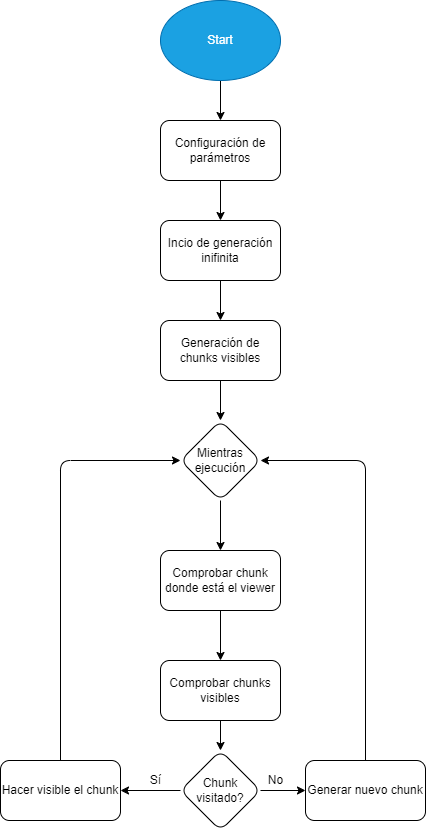
\includegraphics[width=0.6\textwidth]{img/FlowDiagramgeneracionInfinita.png}
    \caption{Diagrama de Flujo de Generación de Terreno.}
\end{figure}


\subsection{Tecnologías y Herramientas Utilizadas}

\subsubsection{Elección de Tecnologías}
Los criterios que se han tenido en cuenta para la elección de las tecnologías específicas para el proyecto son los siguientes:

\begin{itemize}
    \item \textbf{Unity:} El motor de desarrollo que se escogió fue Unity. Se tuvo en cuenta su versatilidad y capacidad para crear aplicaciones interactivas en 3D. Unity proporciona además una amplia gama de herramientas y recursos que facilitan el desarrollo de juegos y simulaciones.
    
    \item \textbf{Unity Job System:} Se utiliza el Unity Job System con el objetivo de optimizar el rendimiento en la generación de terrenos, ya que éste que permite realizar tareas en paralelo utilizando diferentes núcleos de CPU.
    
    \item \textbf{Burst Compiler:} Esta herramienta se utiliza para compilar el código C \# en código nativo muy optimizado, obteniendo una mejora en el rendimiento al generar los terrenos.
    
    \item \textbf{Perlin Noise, Voronoi y Simplex Noise:} Se implementan algoritmos de ruido Perlin, Simplex y Voronoi para la generación de terrenos. Al utilizar estos algoritmos se obtienen unos resultados realistas y variados.
    
\end{itemize}

Estas tecnologías se eligieron con sumo cuidado para obtener un rendimiento óptimo y una gran calidad en la generación de terrenos en tiempo real.

\subsubsection{Lenguajes de Programación}
\begin{itemize}
    \item \textbf{C\#:} El lenguaje de programación utilizado para la realización de este proyecto es C\#. Este es el lenguaje utilizado por los componentes Scripts de Unity de manera que tiene una alta integración con el motor, y es un lenguaje orientado a objetos que ofrece un alto rendimiento, además de su facilidad de uso.
    
\end{itemize}

\subsubsection{Herramientas de Desarrollo}

Para el desarrollo de este proyecto, se utilizaron diversas herramientas y software que tuvieron un papel fundamental en la forma de planificar, implementar y gestionar el trabajo. Las principales herramientas de desarrollo que se utilizaron fueron las siguientes:

\begin{itemize}
    \item \textbf{IDE Principal:} JetBrains Rider fue el IDE principal que se utilizó para la implimentación en C\#. Con Rider, se disponía de un entorno de desarrollo integrado eficiente y potente a la hora de la escritura de código, de la depuración y  de las pruebas realizadas durante el proyecto.
    
    \item \textbf{Visual Studio:} Visual Studio fue utilizado específicamente en la creación de diagramas de clases. Esto permitió representar de manera visual y clara la estructura del proyecto y las relaciones entre las clases.
    
    \item \textbf{VS Code:} Con Visual Studio Code, junto con el plugin draw.io, se crearon varios tipos de diagramas, como los diagramas de casos de uso y diagramas de flujo. Con estas representaciones gráficas se puede comprender y comunicar el flujo de trabajo del sistema. También se usó para la redacción en Latex de la memoria.
        
    \item \textbf{Control de Versiones (Git y GitHub):} Git desempeñó su papel controlando las versiones del código fuente del proyecto. GitHub fue empleado como plataforma de alojamiento del repositorio de Git, lo que facilitó la colaboración en equipo y el seguimiento de cambios.
    
    \item \textbf{Gestión de Tareas (Trello):} Para gestionar las tareas y desarrollar el proyecto se utilizó Trello. Esta herramiento permitió obtener una organización y priorización de las tareas, además de ralizar un seguimiento de cómo avanzaba cada parte del proyecto.

    \item \textbf{Burst Compiler:} Con el Burst Compiler se compiló el código C\# en código nativo muy optimizado. Esto tuvo una contribución significativa en mejorar el rendimiento de la generación de terrenos.
\end{itemize}

Para realizar el proyecto de manera exitosa, estas herramientas tuvieron mucho que ver, ya que proporcionaron las capacidades necesarias para desarrollar y documentar el proyecto, así como para poder colaborar en equipo y optimizar el rendimiento.

\subsubsection{Alternativas Consideradas}
Antes de optar por el diseño final, se tuvieron en cuenta distintas alternativas, incluyendo:

\begin{itemize}
    \item \textbf{Otras Tecnologías de Generación de Terrenos:} Se investigaron distintas tecnologías y enfoques para la generación de terrenos, como el uso de mapas de altura pregenerados en lugar de la generación procedural en tiempo real.
    
    \item \textbf{Métodos de Optimización:} Además del Unity Job System, se tuvieron en cuenta varias técnicas de optimización como el uso de GPU para cálculos intensivos o paralelizar tareas mediante threads manual.
    
    \item \textbf{Otros Algoritmos de Ruido:} Además de Perlin y Simplex, se investigaron otros algoritmos de ruido, eligiendo así los que producían los resultados deseados y optaban por unas mejores técnicas de generación, como el algoritmo diamante-cuadrado. Al final se optó por el ruido debido a que facilitaba la consistencia entre los bordes de partes de terreno nuevas generadas.
\end{itemize}

\subsection{Planificación del Desarrollo}

\subsubsection{Metodología de Desarrollo}
Debido a que la métodología de desarrolló que adoptó el proyecto fue ágil, se pudo mantener una adaptación flexible a medida que se abordaban desafíos técnicos y se tomaban decisiones de diseño. Con el objetivo de planificar y ajustar el enfoque del proyecto, se llevaron a cabo reuniones peiódicas. El repositorio remoto contó con subidas del incremento de desarrollo diarias, teniendo así un control de las mejoras, de cuál era el estado del proyecto y cuáles debían ser los siguientes objetivos.

\subsubsection{Gestión de Tiempo}
La gestión del tiempo se llevó acabo utilizando una planificación detallada en Trello. Se crearon tareas "por hacer", "en desarrollo", "terminadas" y "mejorables".

La planificación del proyecto se ha desglosado en las siguientes fases. Estas fases culminan con sus correspondientes hitos.
\begin{itemize}
    \item \textbf{Análisis preeliminar}: Esta fase es la encargada de determinar los objetivos, los requisitos y el alcance del proyecto. Se hace una investigación acerca de los recursos que se podrán emplear y finalizará con el hito de la aprobación del análisis preeliminar.
    \item \textbf{Fase de Análisis}: Como su propio nombre indica, esta fase se corresponde con el análisis del proyecto: Se estudian los requisitos, la arquitectura que se va a diseñar y los procesos y componentes que se llevarán a cabo en el proyecto. El hito que da por finalizada esta fase es la aprobación del análisis.
    \item \textbf{Fase de Diseño}: En la fase de diseño se encargará de diseñar la estructura de la arquitectura que se otorgará a la herramienta, las relaciones entre los distintos componentes, y los parámetros que el usuario facilitará para la generación del terreno. Esta fase culmina con la aprobación del diseño.
    \item \textbf{Implementación}: Durante esta fase se llevará a cabo la implementación de todos los componentes, clases y procesos necesarios. Acaba cuando se lleva a cabo el comienzo de las pruebas.
    \item \textbf{Pruebas y resultados}: Aquí se desarrollan diferentes pruebas y correcciones sobre la implementación anteriormente llevada a cabo. Esta fase acaba con la aprobación de los resultados de las últimas pruebas realizadas.
    \item \textbf{Finalización de la documentación}: El hito de la finalización de la documentación se produce con la entrega de la memoria y el video explicativo de este proyecto.
\end{itemize}

El cronograma de desarrollo se puede encontrar detallado en el apéndice A para una referencia más completa.

\subsubsection{Recursos Necesarios}
Para llevar a cabo el desarrollo del proyecto se utilizaron los siguientes recursos:

\begin{itemize}
    \item \textbf{Personal de Desarrollo}: El personal que trabajó en el proyecto fue una única persona que se ocupó de todos los roles del desarrollo, tanto diseñador, como analista, como desarrollador como jefe de equipo. Además, tomó parte un product owner que se encargaba de especificar los requisitos que debía cumplir el proyecto.
    
    \item \textbf{Hardware}: El equipo que se utilizó fue un equipo portátil con procesador i5-11400H con 2.7GHz, 16 GB de RAM, 1TB de memoria en disco y tarjeta gráfica NVidia 3060 con 6GB de RAM. El equipo contaba con windows 10 Home como sistema operativo. 
    
    \item \textbf{Software}: Se requirieron herramientas como Unity, JetBrains Rider, Visual Studio, VS Code con el plugin draw.io, LaTeX y el Burst Compiler para el desarrollo y la documentación del proyecto.
\end{itemize}

